\chapter{Resultate}
\label{ch:results}

In diesem Kapitel stellen wir die quantitativen Resultate aus den fünf Entwicklungsphasen vor. Die Daten stammen aus den MLflow-Tracking-Aufzeichnungen sowie den Evaluierungsläufen der jeweiligen Modellvarianten.

\section{Vergleich der Entwicklungsphasen}
Über den gesamten Projektverlauf hinweg haben wir die Performance der verschiedenen Modellarchitekturen systematisch erfasst. In \autoref{tab:phase_accuracy} sehen Sie, wie sich die Genauigkeit (Accuracy) von der statischen Vorphase bis hin zum finalen Transformer-Modell entwickelt hat.

\begin{table}[h]
\centering
\caption{Übersicht der erreichten Genauigkeiten pro Phase}
\label{tab:phase_accuracy}
\begin{tabular}{cllr}
\toprule
Phase & Architektur & Fokus & Validierungsgüte \\
\midrule
1 & CNN & Statisches Alphabet (25 Klassen) & 99,60 \% \\
2 & Transformer v1 & Dynamische Gebärden (146 Klassen) & 53,94 \% \\
3 & Skeleton-Graph & Anatomische Graphen-Pipeline & 31,56 \% \\
4 & Transformer v2 & Self-Attention Baseline & 66,61 \% \\
5 & Transformer Final & Optimiertes Feature Engineering & 73,86 \% \\
\bottomrule
\end{tabular}
\end{table}

\section{Analyse des Trainingsverlaufs}
Um die Stabilität und Konvergenz des finalen Modells (Phase 5) zu prüfen, haben wir den Verlauf von Loss und Accuracy während des Trainings aufgezeichnet.

\begin{figure}[htbp]
    \centering
    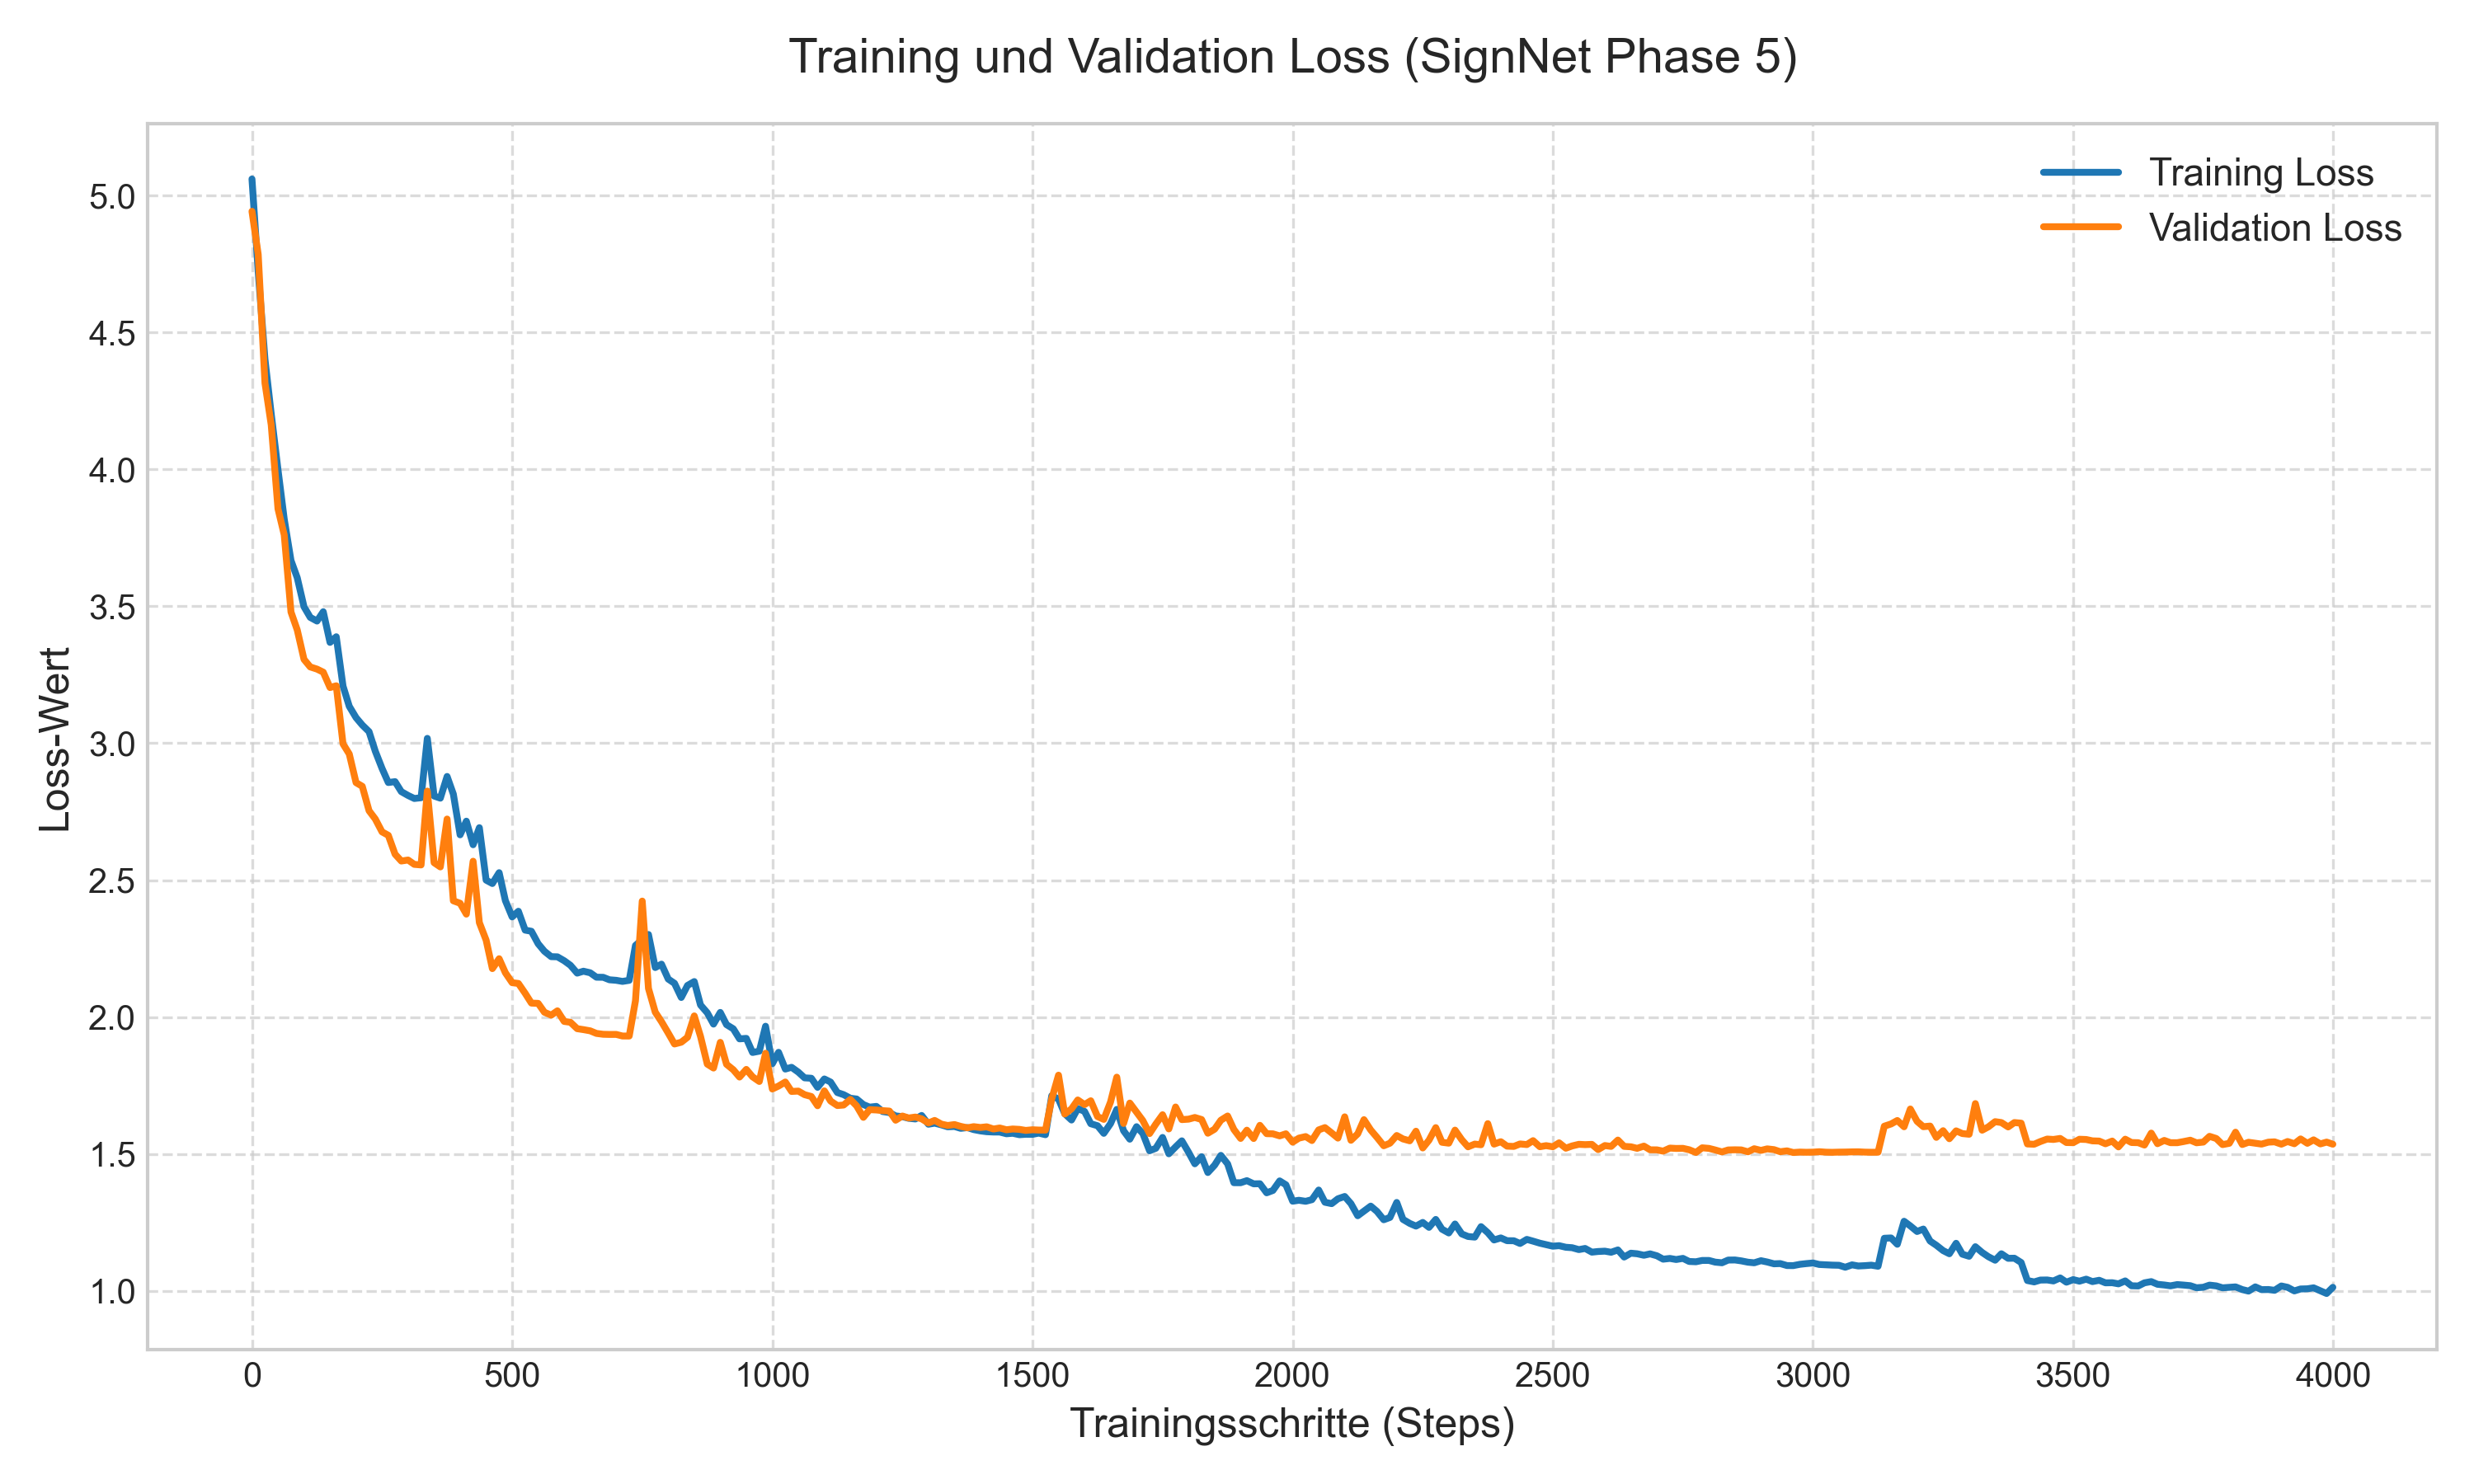
\includegraphics[width=0.85\textwidth]{figures/loss_plot_final.png}
    \caption{Verlauf von Trainings- und Validierungs-Loss: Die stetige Abnahme beider Kurven ohne Divergenz deutet auf eine gute Generalisierung hin.}
    \label{fig:loss_plot}
\end{figure}

\begin{figure}[htbp]
    \centering
    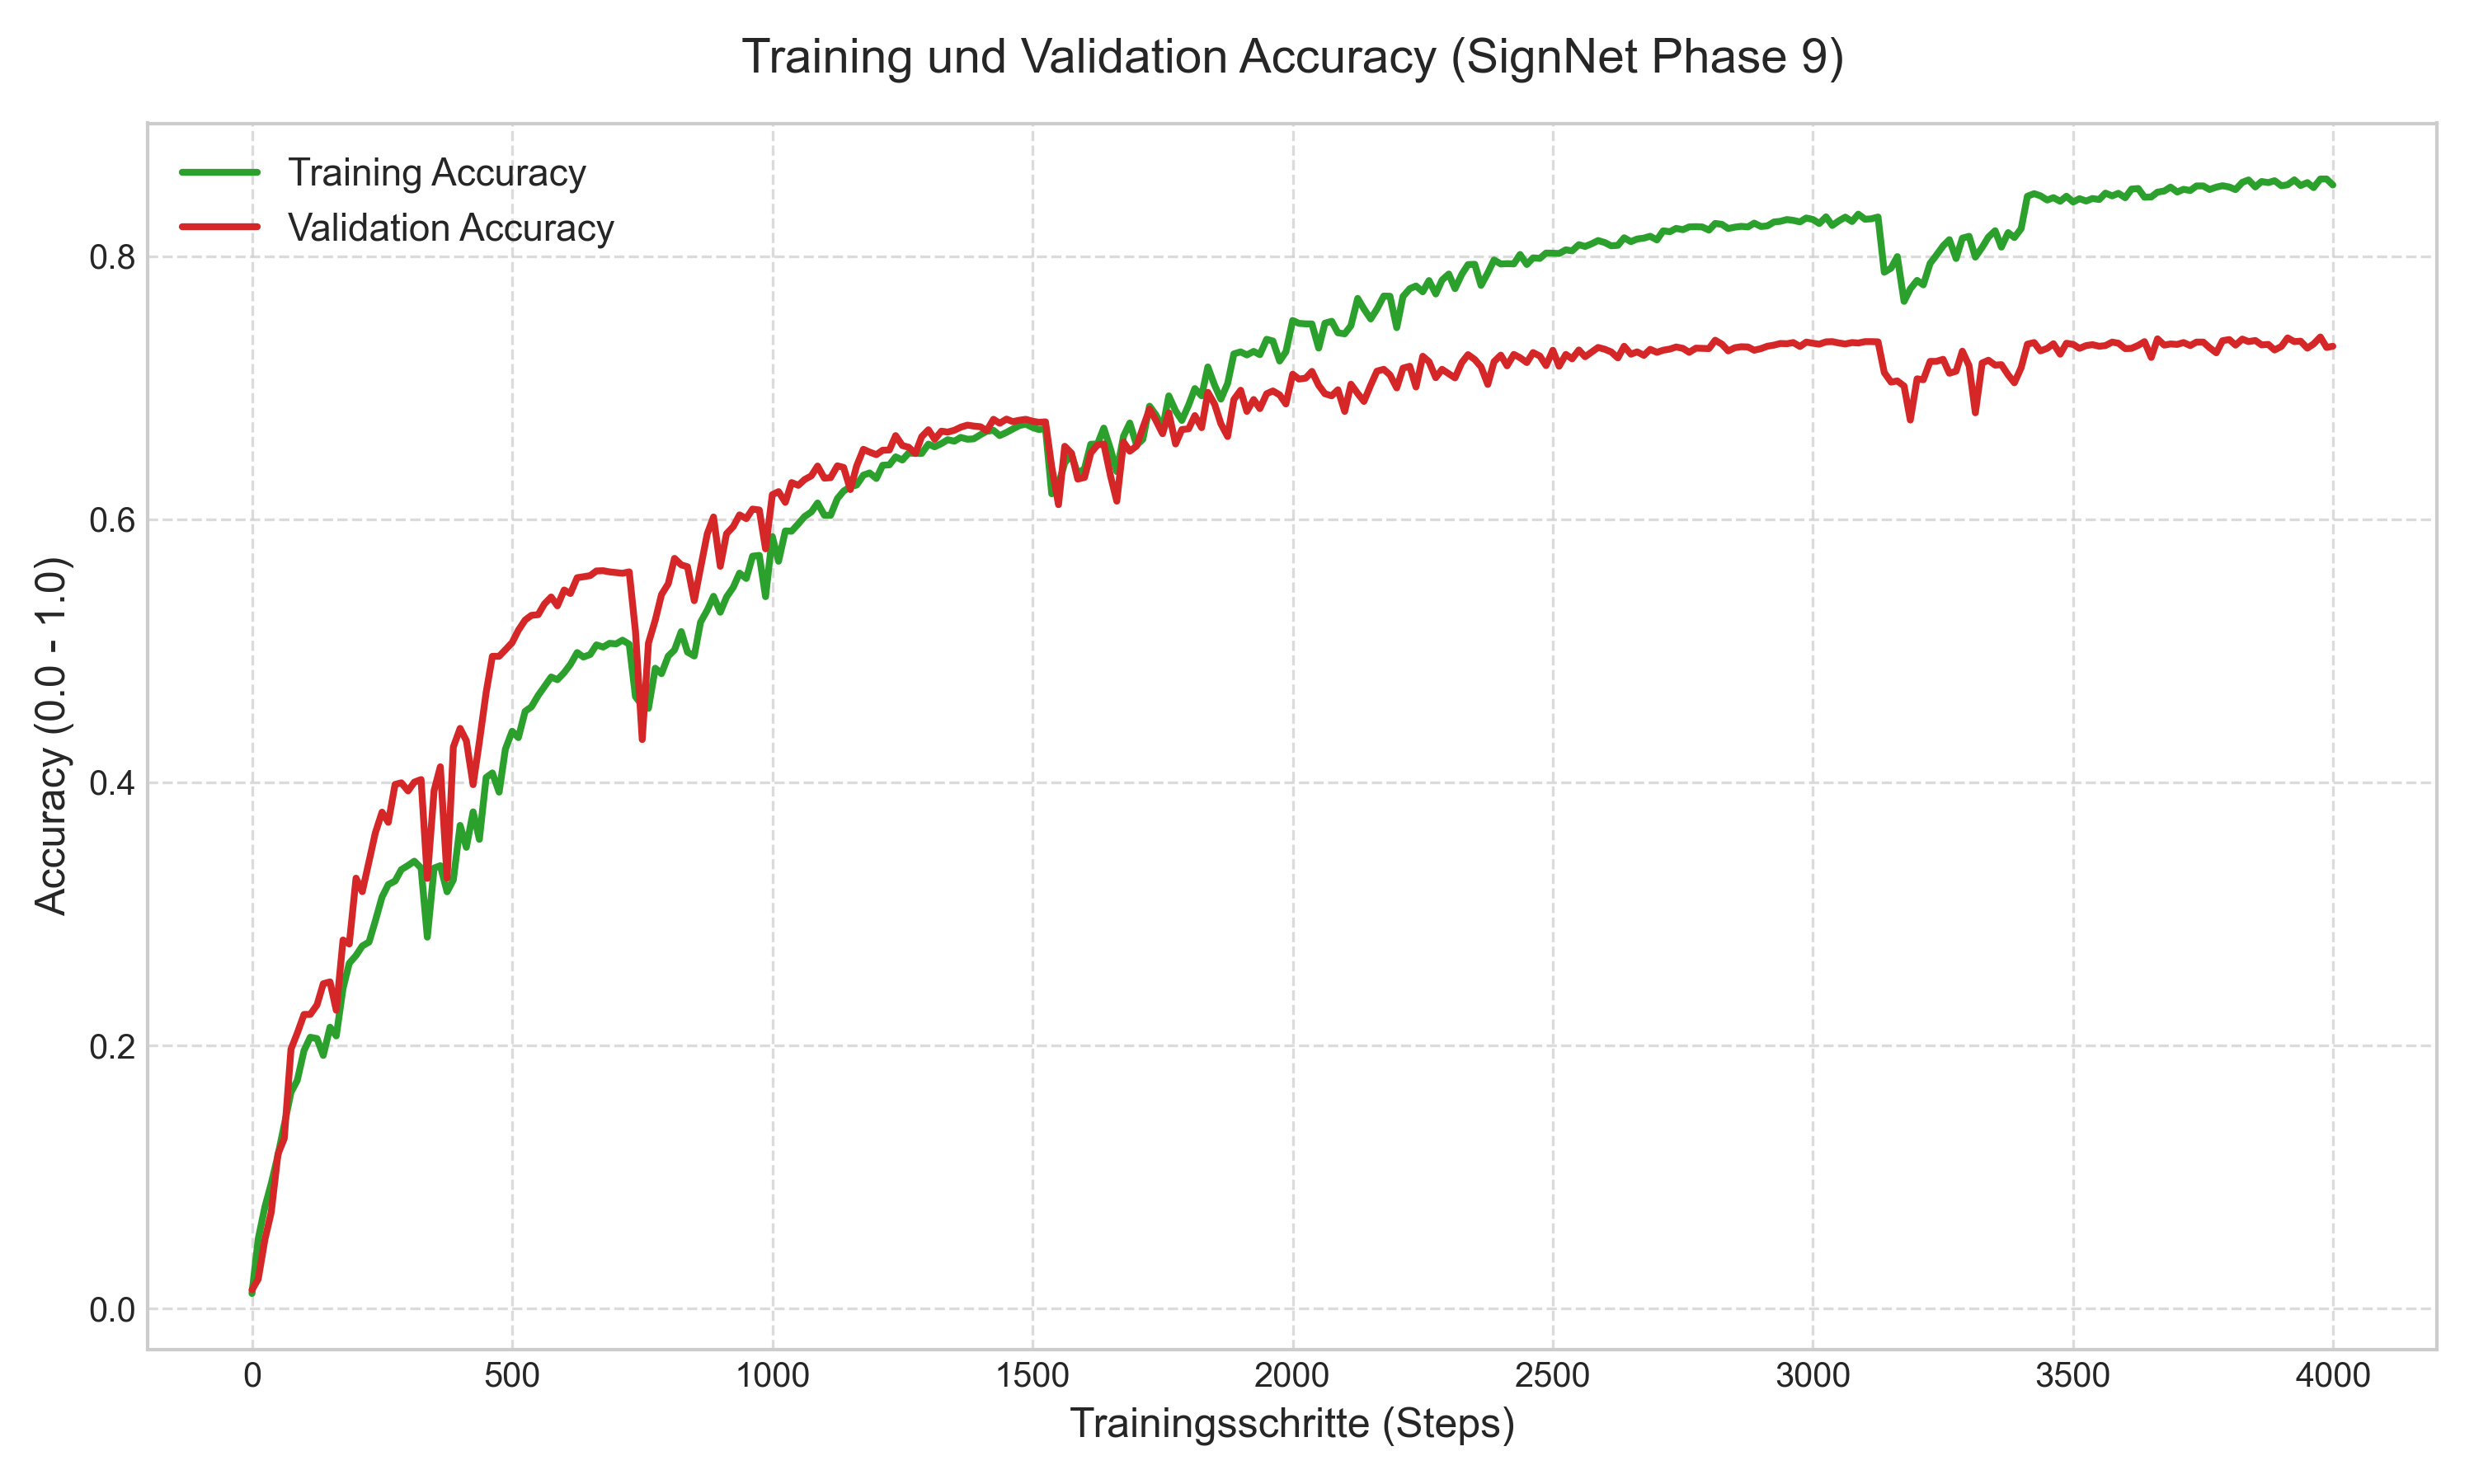
\includegraphics[width=0.85\textwidth]{figures/accuracy_plot_final.png}
    \caption{Entwicklung der Trainings- und Validierungs-Accuracy über die Trainingsschritte.}
    \label{fig:accuracy_plot}
\end{figure}

Wie in \autoref{fig:loss_plot} ersichtlich, konvergieren Trainings- und Validierungsverlust stabil. Die Accuracy (\autoref{fig:accuracy_plot}) steigt parallel an, wobei die geringe Differenz zwischen den Kurven die Wirksamkeit der gewählten Regularisierungsmaßnahmen (Dropout 0,65) bestätigt.

\section{Quantitative Ergebnisse}
Die Modellleistung wurde anhand der Top-1- und Top-5-Accuracy bewertet. Bei einem Vokabular von 146 Klassen haben wir folgende Werte erreicht:

\begin{table}[h]
\centering
\caption{Globale Klassifikationsergebnisse (Phase 5)}
\label{tab:globale_ergebnisse}
\begin{tabular}{lr}
\toprule
Metrik & Wert \\
\midrule
Top-1 Accuracy & \textbf{73,86 \%} \\
Top-5 Accuracy & \textbf{91,76 \%} \\
Anzahl Test-Samples & 4.489 \\
Klassenanzahl ($N \ge 70$) & 146 \\
\bottomrule
\end{tabular}
\end{table}

Die hohe Top-5-Genauigkeit von über 91\,\% zeigt, dass das System in den meisten Fällen die richtige Gebärde unter den wahrscheinlichsten Kandidaten identifiziert – ein wichtiger Aspekt für den praktischen Einsatz in interaktiven Übersetzungssystemen.

\section{Konfidenz-Analyse und Kalibrierung}
Zur Bewertung der Vorhersagezuverlässigkeit haben wir die Softmax-Konfidenz untersucht. Die Ergebnisse zeigen eine klare Trennung zwischen sicheren und unsicheren Vorhersagen:

\begin{table}[h]
\centering
\caption{Statistische Auswertung der Modell-Konfidenz}
\label{tab:konfidenz_stats}
\begin{tabular}{lr}
\toprule
Kategorie & Durchschnittliche Konfidenz \\
\midrule
Korrekte Vorhersagen & \textbf{87,37 \%} \\
Fehlklassifikationen & \textbf{57,19 \%} \\
\midrule
Anteil „Sichere Fehler“ (Konfidenz $> 0,8$) & 5,30 \% \\
\bottomrule
\end{tabular}
\end{table}

\begin{figure}[htbp]
    \centering
    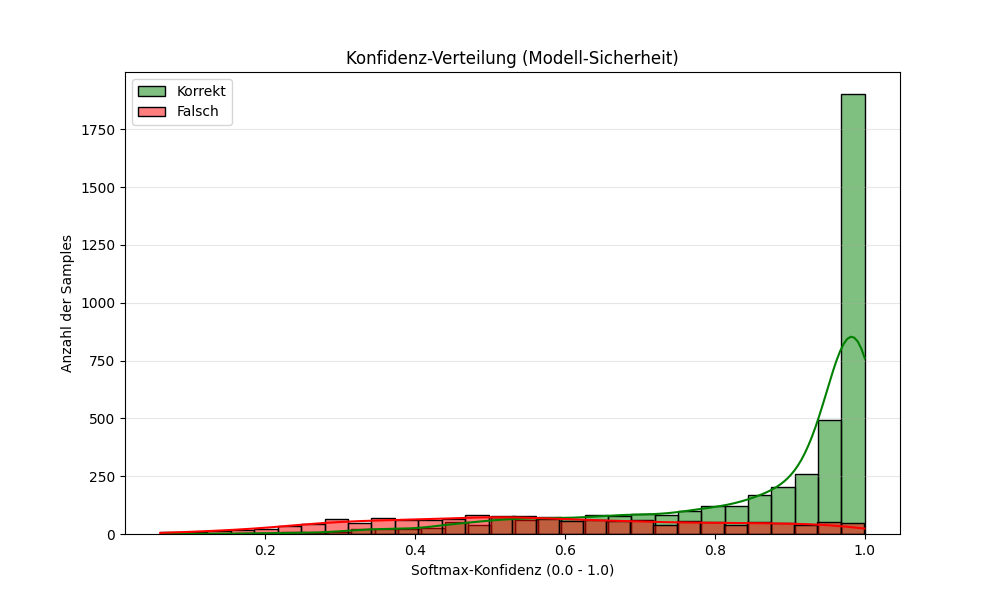
\includegraphics[width=1.0\textwidth]{figures/confidence_distribution.png}
    \caption{Konfidenz-Verteilung der Vorhersagen: Gegenüberstellung von korrekten (grün) und falschen (rot) Klassifizierungen zur Bewertung der Modell-Kalibrierung.}
    \label{fig:confidence_dist}
\end{figure}

Die Verteilung in \autoref{fig:confidence_dist} macht deutlich: korrekte Klassifizierungen liegen meist nahe bei 1,0, während Fehler deutlich unsicherer sind.

\section{Detaillierte Fehleranalyse}
Trotz der insgesamt robusten Performance gibt es systematische Verwechslungen. Die Konfusionsmatrix in \autoref{fig:confusion_matrix} zeigt die zehn Klassen mit dem niedrigsten F1-Score und dient als Grundlage für die linguistische Diskussion im nächsten Kapitel.

\subsection{Visualisierung der Fehlklassifikationen}
\autoref{fig:confusion_matrix} zeigt die Konfusionsmatrix für die 10 Klassen mit der geringsten Trennschärfe.

\begin{figure}[htbp]
    \centering
    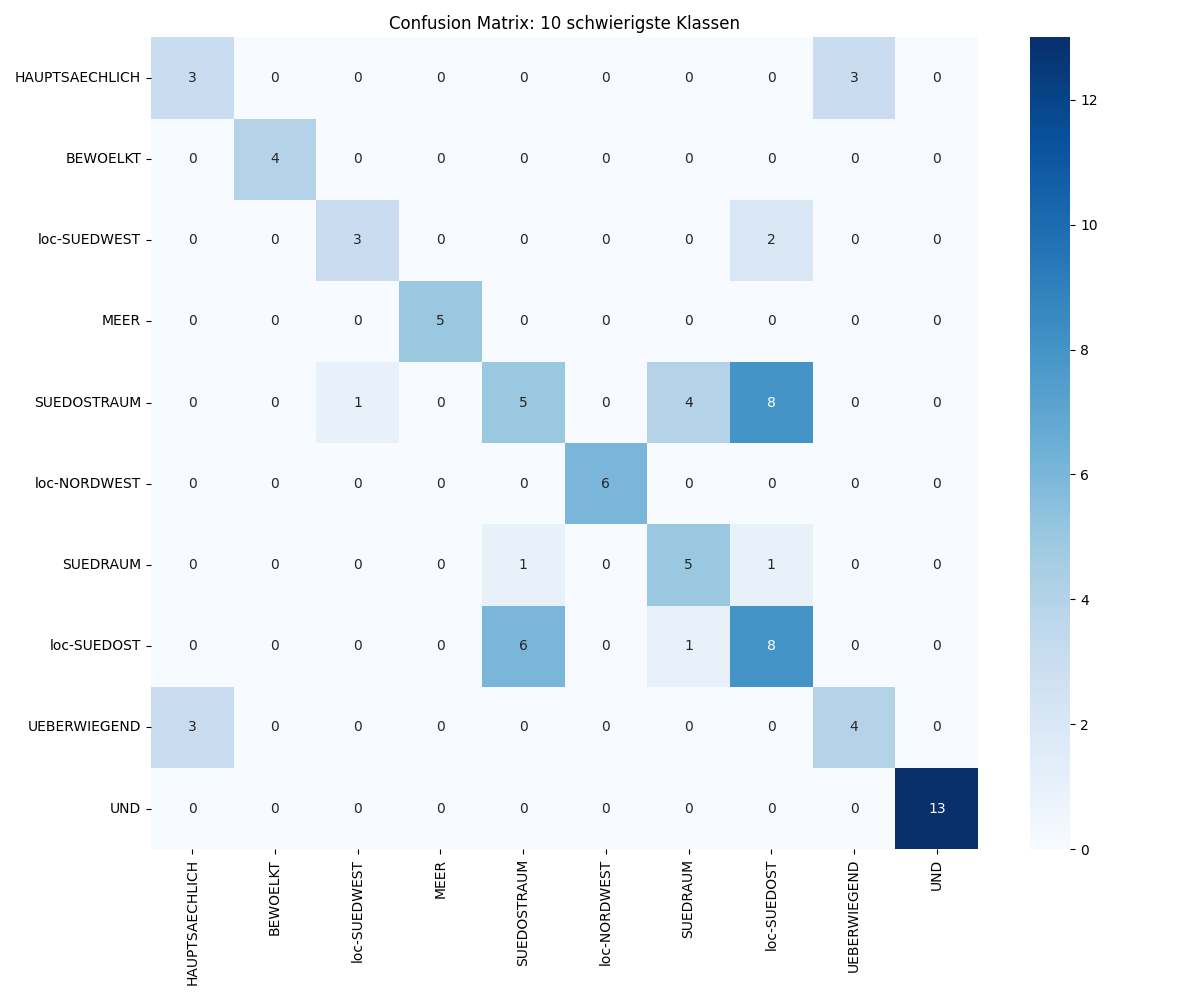
\includegraphics[width=1.0\textwidth]{figures/confusion_matrix_worst10.png}
    \caption{Konfusionsmatrix der 10 Klassen mit der geringsten Trennschärfe. Die Diagonale repräsentiert korrekte Vorhersagen, während die Nebenwerte die systematischen Verwechslungen innerhalb semantischer Gruppen visualisieren.}
    \label{fig:confusion_matrix}
\end{figure}